\chapter{Ondes sonores}

\newpage

\section{Impédance acoustique}

On s'intéresse à la propagation d'une onde sonore dans un milieu ayant une masse volumique au repos $\rho_0$ et une compressibilité $\chi_s$. Dans tout l'exercice, on considèrera que l'onde se propage unidimensionnellement selon l'axe $\vec{e}_x$. Les vibrations des ondes sonores sont caractérisées par des variations locales du champ de pression $P = P_0 + p(x,t)$, de masse volumique $\rho=\rho_0 + \mu(x,t)$ et de vitesse $\vec{v}=v(x,t)\vec{e}_x$. 

\begin{enumerate}

\item 

\begin{enumerate}

	\item Établir deux équations différentielles couplées entre $\vec{v}(x,t)$ et $p(x,t)$.
	
	\item En déduire l'équation d'Alembert vérifiée par la surpression $p(x,t)$ et la vitesse $\vec{v}(x,t)$ dans un milieu homogène, et expliciter une vitesse $c_0$. Quelles sont les solutions générales dans ce cas unidimensionnel ? 

\end{enumerate}
	
\item On s'intéresse désormais au cas où le milieu de propagation n'est plus homogène, mais est constitué de deux milieux 1 et 2, caractérisés par leur masse volumique $\rho_1$ et $\rho_2$. Le demi-espace $x<0$ est constitué du milieu 1, et le demi-espace $x>0$ est constitué du milieu 2. On écrit les solutions des champs de vitesse et de surpression de l'équation d'Alembert comme : 
\begin{align*}
	v_j(x,t)&=v^+_{j}\left( t-\frac{x}{c_j}\right) + v^-_{j}\left( t+\frac{x}{c_j}\right) \\
	p_j(x,t)&=p^+_{j}\left( t-\frac{x}{c_j}\right) + p^-_{j}\left( t+\frac{x}{c_j}\right) 
\end{align*}
où l'indice $j$ représente le milieu 1 ou 2. Pour simplifier, on a supposé que le vecteur vitesse $\vec{v}_j(x,t)=v_j(x,t)\vec{e}_x$ n'a de composante que sur $x$ pour s'affranchir de la notation vectorielle. 

\begin{enumerate}
	
	\item Donner la signification physique du signe $+$ et $-$ dans l'écriture des champs. Trouver deux relations, une entre $v^+_{j}$ et $p^+_{j}$ et une autre entre $v^-_{j}$ et $p^-_{j}$. On fera intervenir l'impédance acoustique du milieu $Z_j=c_j\rho_j$.
	
	\item Quelle relations que vérifient la vitesse et la surpression à l'interface en $x=0$ ? Justifier. 
	
	\item Quelqu'un génère une onde depuis les $x<0$, qui arrive sur l'interface depuis le milieu 1. Pourquoi a t-on nécessairement l'apparition d'une onde réfléchie et d'une onde transmise à l'interface si les milieux 1 et 2 ne sont pas les mêmes ?
	
	\item Exprimer les coefficients de réflexion en vitesse $r_v=v_1^-(t)/v_1^+(t)$ et de transmission $t_v=v_2^+(t)/v_1^+(t)$, puis les coefficients de réflexion en pression $r_p$ et de transmission $t_p$
	
	\item En déduire les coefficients de réflexion $R$ et de transmission $T$ en intensité. 
	
	\item Pourquoi dont-on mettre un gel sur entre la sonde et le corps durant une échographie ? 
		
\end{enumerate}

\end{enumerate}

\newpage

\begin{correction}

\begin{enumerate}

\item

\begin{enumerate}

\item On commence par l'équation d'Euler qui donne une première relation entre $v$ et $p$ :
	\begin{align*}
		 \rho_0\frac{\partial \vec{v}}{\partial t}+\vec{\mathrm{grad}}(P) &=0 \\
		 \rho_0\frac{\partial v}{\partial t}+\frac{\partial p}{\partial x} &=0	
	\end{align*}

	Ensuite, l'équation de la conservation de la masse :
	\begin{align*} 
		\frac{\partial \rho}{\partial t}+\mathrm{div}(\vec{v})&=0 \\
		\frac{\partial \mu}{\partial t}+\frac{\partial v}{\partial x}&=0
	\end{align*}
	Pour trouver une relation entre la masse volumique et la pression, on utilise la compressibilité :
	\begin{align*}
		\chi&=-\frac{1}{V}\frac{\partial V}{\partial P} \\
		\chi&=-\rho_0\left(\frac{\mu}{\rho_0^2}\frac{1}{p} \right) \\
		\mu &= \chi_sp\rho_0
	\end{align*}
	On obtient donc deux équations couplées :
	\begin{align*}
		\rho_0\frac{\partial v}{\partial t}&=-\frac{\partial p}{\partial x} \\
		\chi_S\frac{\partial p}{\partial t}&=-\frac{\partial v}{\partial x}
	\end{align*}
	
	\item Avec les deux équations précédentes, on obtient l'équation d'Alembert sur la vitesse ou la surpression :
	\begin{align*}
		\frac{\partial^2 v}{\partial t^2}=\frac{1}{c_0^2}\frac{\partial^2v}{\partial x^2}
	\end{align*}
	La célérité est $c_0=1/\sqrt{\chi_s\rho_0}$.

\end{enumerate}

\item

\end{enumerate}

\item $v^+_{j}$ et $v^-_{j}$ sont les champs de vitesse se propageant respectivement suivant les $x$ croissants et décroissants. Ils sont indépendants l'un de l'autre : on peut avoir une onde incidente sans onde réfléchie ($v^+_{j}\neq0$ et $v^-_{j}=0$) et vice-versa. Même chose pour la surpression.

En injectant dans une des équations couplées précédentes, on a alors :
\begin{align*}
		\rho_0\left(v'^+_{j}+v'^-_{j}\right) &=-\frac{1}{c_j}\left(-p'^+_{j}+p'^-_{j}\right)
\end{align*}

\item 

\end{correction}

\newpage

\section{Onde acoustique guidée}

Un émetteur produit dans l'air une onde acoustique de fréquence $f=40$kHz et de longueur d'onde $\lambda$. L'air possède une masse molaire $M=29$g.mol$^{-1}$, un coefficient de compressibilité isentropique $\chi_S$ et un coefficient de Laplace $\gamma$. Au repos, à $20^\circ C$, la pression de l'air vaut $P_0=1$bar et sa masse volumique $\mu_0=1,2$kg.m$^{-3}$.
Au passage de l'onde sonore, que l'on suppose se propager uniquement suivant l'axe $x$, les grandeurs thermodynamique de l'air sont modifiées : $\mu=\mu_0+\mu_1(x,t)$, $P=P_0+P_1(x,t)$ et $\vec{v}=v(x,t)\vec{e}_x$.

\begin{enumerate}

    \item Qu'est-ce que l'approximation acoustique ? En déduire trois équations linéarisées reliant $\mu_1$, $p_1$ et $v$ ainsi que les données de l'énoncé. 

    \item En déduire l'équation d'onde vérifiée par la surpression $p_1(x,t)$. 

    \item Pour une OPPM, établir l'expression de l'impédance acoustique $Z_a$. Exprimer l'intensité en décibel $I_{dB}$ en fonction de $v_m$ l'amplitude de la vitesse acoustique, $I_0=1,0\times10^{-12}$W.m$^{-2}$ l'intensité seuil d'audibilité d'un son, et $Z_a$. Calculer numériquement $v_m$ si $I_{dB}=120$dB.

    \item On généralise l'équation d'onde à deux dimensions :
    \begin{align*}
        \frac{\partial^2 p_1(M,t)}{\partial t^2}(M,t)=c^2\Delta p_1(M,t)
    \end{align*}
    Et on suppose désormais que deux plaques rigides de grandes dimensions sont fixées en $z=0$ et en $z=a$. Elles imposent comme conditions à la surpression : 
    \begin{align*}
        \left.\frac{\partial p_1}{\partial z}\right|_{z=0}=\left.\frac{\partial p_1}{\partial z}\right|_{z=a}=0
    \end{align*}

\begin{center}
	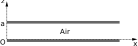
\includegraphics[scale=0.8]{onde_sonore1.pdf}
\end{center}

    On cherche une solution du problème sous la forme $p_1(M,t)=p(z)\cos(\omega t-kx +\Phi)$. Décrire physiquement cette onde.

    \item Déterminer l'équation différentielle vérifiée par $p(z)$. On montrera que les solutions s'écrivent :
    \begin{align*}
        p_n(z)=A_n\cos\left(\frac{n\pi}{a}z\right)
    \end{align*}
    où $n$ est un entier.

    \item Trouver la relation de dispersion pour chaque mode $n$ et montrer l'existence d'une pulsation de coupure $\omega_{c,n}$ à partir de laquelle le mode $n>0$ peut se propager. 

    \item A quelle condition sur $a$ et la longueur d'onde $\lambda$ de l'onde libre, le mode fondamental $n=0$ se propage t-il seul entre les plaques ? Faire l'application numérique. 



\end{enumerate}